\documentclass{standalone}
\usepackage{tikz}
\usetikzlibrary{patterns, positioning}
\usepackage[sfdefault]{ClearSans} %% option 'sfdefault' activates Clear Sans as the default text font
\usepackage[T1]{fontenc}

\begin{document}
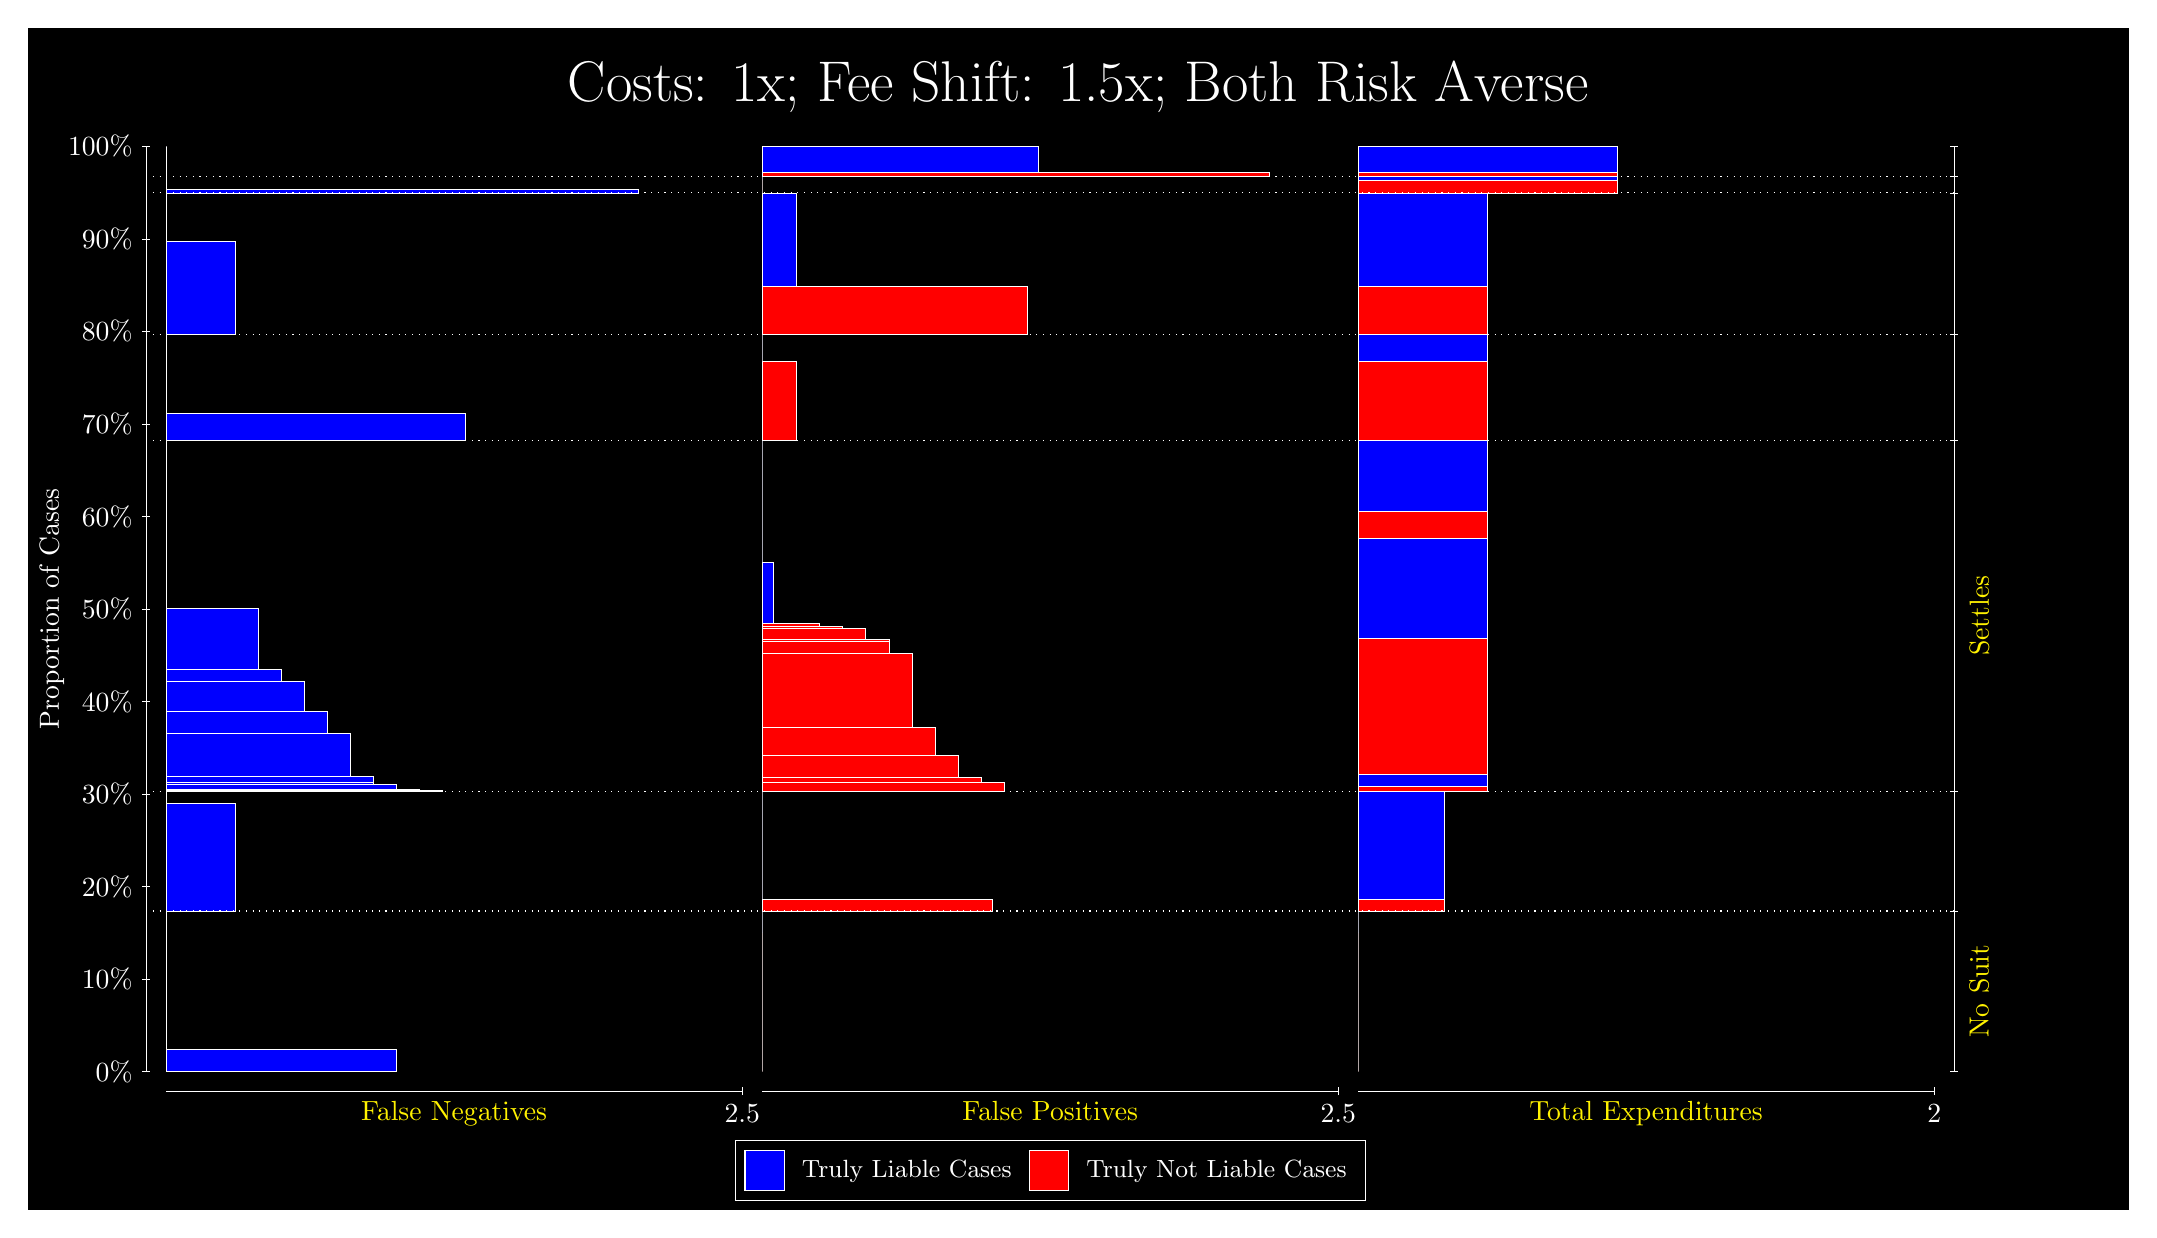
\begin{tikzpicture}
\draw[fill=black] (0,0) rectangle (26.667,15);
\draw[text=white] (0,13.5) rectangle (26.667,15) node[midway] {\huge Costs: 1x; Fee Shift: 1.5x; Both Risk Averse};
\draw[white, very thin] (1.5,1.75) -- (1.5,13.5);
\node[rotate=90, text=white, anchor=center] at (0.3, 7.625) {Proportion of Cases};
\draw[white, very thin] (1.45,1.75) -- (1.55,1.75);
\node[text=white, anchor=east] at (1.45, 1.75) {0\%};
\draw[white, very thin] (1.45,2.925) -- (1.55,2.925);
\node[text=white, anchor=east] at (1.45, 2.925) {10\%};
\draw[white, very thin] (1.45,4.1) -- (1.55,4.1);
\node[text=white, anchor=east] at (1.45, 4.1) {20\%};
\draw[white, very thin] (1.45,5.275) -- (1.55,5.275);
\node[text=white, anchor=east] at (1.45, 5.275) {30\%};
\draw[white, very thin] (1.45,6.45) -- (1.55,6.45);
\node[text=white, anchor=east] at (1.45, 6.45) {40\%};
\draw[white, very thin] (1.45,7.625) -- (1.55,7.625);
\node[text=white, anchor=east] at (1.45, 7.625) {50\%};
\draw[white, very thin] (1.45,8.8) -- (1.55,8.8);
\node[text=white, anchor=east] at (1.45, 8.8) {60\%};
\draw[white, very thin] (1.45,9.975) -- (1.55,9.975);
\node[text=white, anchor=east] at (1.45, 9.975) {70\%};
\draw[white, very thin] (1.45,11.15) -- (1.55,11.15);
\node[text=white, anchor=east] at (1.45, 11.15) {80\%};
\draw[white, very thin] (1.45,12.325) -- (1.55,12.325);
\node[text=white, anchor=east] at (1.45, 12.325) {90\%};
\draw[white, very thin] (1.45,13.5) -- (1.55,13.5);
\node[text=white, anchor=east] at (1.45, 13.5) {100\%};

\draw[white, very thin] (24.457,1.75) -- (24.457,13.5);
\draw[white, very thin] (24.407,1.75) -- (24.507,1.75);
\node[anchor=west] at (24.407, 1.75) {};
\draw[white, very thin] (24.407,3.7888) -- (24.507,3.7888);
\node[anchor=west] at (24.407, 3.7888) {};
\draw[white, very thin] (24.407,5.312) -- (24.507,5.312);
\node[anchor=west] at (24.407, 5.312) {};
\draw[white, very thin] (24.407,9.7639) -- (24.507,9.7639);
\node[anchor=west] at (24.407, 9.7639) {};
\draw[white, very thin] (24.407,11.114) -- (24.507,11.114);
\node[anchor=west] at (24.407, 11.114) {};
\draw[white, very thin] (24.407,12.908) -- (24.507,12.908);
\node[anchor=west] at (24.407, 12.908) {};
\draw[white, very thin] (24.407,13.122) -- (24.507,13.122);
\node[anchor=west] at (24.407, 13.122) {};
\draw[white, very thin] (24.407,13.5) -- (24.507,13.5);
\node[anchor=west] at (24.407, 13.5) {};

\draw[white, very thin, fill=blue] (1.75,1.75) rectangle (4.6775,2.0268);
\draw[white, very thin, fill=red] (1.75,2.0268) rectangle (1.75,3.7888);
\draw[white, very thin, fill=blue] (1.75,3.7888) rectangle (2.6283,5.1574);
\draw[white, very thin, fill=red] (1.75,5.1574) rectangle (1.75,5.312);
\draw[white, very thin, fill=blue] (1.75,5.312) rectangle (5.2631,5.3242);
\draw[white, very thin, fill=blue] (1.75,5.3242) rectangle (4.9703,5.3354);
\draw[white, very thin, fill=blue] (1.75,5.3354) rectangle (4.6775,5.4007);
\draw[white, very thin, fill=blue] (1.75,5.4007) rectangle (4.3848,5.428);
\draw[white, very thin, fill=blue] (1.75,5.428) rectangle (4.3848,5.4953);
\draw[white, very thin, fill=blue] (1.75,5.4953) rectangle (4.092,6.0483);
\draw[white, very thin, fill=blue] (1.75,6.0483) rectangle (3.7993,6.3193);
\draw[white, very thin, fill=blue] (1.75,6.3193) rectangle (3.5065,6.7009);
\draw[white, very thin, fill=blue] (1.75,6.7009) rectangle (3.2138,6.8542);
\draw[white, very thin, fill=blue] (1.75,6.8542) rectangle (2.921,7.6329);
\draw[white, very thin, fill=red] (1.75,7.6329) rectangle (1.75,9.7639);
\draw[white, very thin, fill=blue] (1.75,9.7639) rectangle (5.5558,10.115);
\draw[white, very thin, fill=red] (1.75,10.115) rectangle (1.75,11.114);
\draw[white, very thin, fill=blue] (1.75,11.114) rectangle (2.6283,12.295);
\draw[white, very thin, fill=red] (1.75,12.295) rectangle (1.75,12.908);
\draw[white, very thin, fill=blue] (1.75,12.908) rectangle (7.7515,12.959);
\draw[white, very thin, fill=red] (1.75,12.959) rectangle (1.75,13.122);
\draw[white, very thin, fill=red] (1.75,13.122) rectangle (1.75,13.174);
\draw[white, very thin, fill=blue] (1.75,13.174) rectangle (1.75,13.5);
\draw[white, very thin, fill=red] (9.3189,1.75) rectangle (9.3189,3.512);
\draw[white, very thin, fill=blue] (9.3189,3.512) rectangle (9.3189,3.7888);
\draw[white, very thin, fill=red] (9.3189,3.7888) rectangle (12.246,3.9434);
\draw[white, very thin, fill=blue] (9.3189,3.9434) rectangle (9.3189,5.312);
\draw[white, very thin, fill=red] (9.3189,5.312) rectangle (12.393,5.4237);
\draw[white, very thin, fill=red] (9.3189,5.4237) rectangle (12.1,5.4887);
\draw[white, very thin, fill=red] (9.3189,5.4887) rectangle (11.807,5.7711);
\draw[white, very thin, fill=red] (9.3189,5.7711) rectangle (11.515,6.1177);
\draw[white, very thin, fill=red] (9.3189,6.1177) rectangle (11.222,7.0605);
\draw[white, very thin, fill=red] (9.3189,7.0605) rectangle (10.929,7.2116);
\draw[white, very thin, fill=red] (9.3189,7.2116) rectangle (10.929,7.2412);
\draw[white, very thin, fill=red] (9.3189,7.2412) rectangle (10.636,7.376);
\draw[white, very thin, fill=red] (9.3189,7.376) rectangle (10.344,7.4034);
\draw[white, very thin, fill=red] (9.3189,7.4034) rectangle (10.051,7.4431);
\draw[white, very thin, fill=blue] (9.3189,7.4431) rectangle (9.4652,8.2217);
\draw[white, very thin, fill=blue] (9.3189,8.2217) rectangle (9.3189,9.7639);
\draw[white, very thin, fill=red] (9.3189,9.7639) rectangle (9.758,10.764);
\draw[white, very thin, fill=blue] (9.3189,10.764) rectangle (9.3189,11.114);
\draw[white, very thin, fill=red] (9.3189,11.114) rectangle (12.686,11.727);
\draw[white, very thin, fill=blue] (9.3189,11.727) rectangle (9.758,12.908);
\draw[white, very thin, fill=red] (9.3189,12.908) rectangle (9.3189,13.071);
\draw[white, very thin, fill=blue] (9.3189,13.071) rectangle (9.3189,13.122);
\draw[white, very thin, fill=red] (9.3189,13.122) rectangle (15.759,13.174);
\draw[white, very thin, fill=blue] (9.3189,13.174) rectangle (12.832,13.5);
\draw[white, very thin, fill=red] (16.888,1.75) rectangle (16.888,3.512);
\draw[white, very thin, fill=blue] (16.888,3.512) rectangle (16.888,3.7888);
\draw[white, very thin, fill=red] (16.888,3.7888) rectangle (17.986,3.9434);
\draw[white, very thin, fill=blue] (16.888,3.9434) rectangle (17.986,5.312);
\draw[white, very thin, fill=red] (16.888,5.312) rectangle (18.534,5.377);
\draw[white, very thin, fill=blue] (16.888,5.377) rectangle (18.534,5.5304);
\draw[white, very thin, fill=red] (16.888,5.5304) rectangle (18.534,7.2533);
\draw[white, very thin, fill=blue] (16.888,7.2533) rectangle (18.534,8.5262);
\draw[white, very thin, fill=red] (16.888,8.5262) rectangle (18.534,8.8693);
\draw[white, very thin, fill=blue] (16.888,8.8693) rectangle (18.534,9.7639);
\draw[white, very thin, fill=red] (16.888,9.7639) rectangle (18.534,10.764);
\draw[white, very thin, fill=blue] (16.888,10.764) rectangle (18.534,11.114);
\draw[white, very thin, fill=red] (16.888,11.114) rectangle (18.534,11.727);
\draw[white, very thin, fill=blue] (16.888,11.727) rectangle (18.534,12.908);
\draw[white, very thin, fill=red] (16.888,12.908) rectangle (20.181,13.071);
\draw[white, very thin, fill=blue] (16.888,13.071) rectangle (20.181,13.122);
\draw[white, very thin, fill=red] (16.888,13.122) rectangle (20.181,13.174);
\draw[white, very thin, fill=blue] (16.888,13.174) rectangle (20.181,13.5);
\draw[white, dotted] (1.5,3.7888) -- (24.457,3.7888);
\draw[white, dotted] (1.5,5.312) -- (24.457,5.312);
\draw[white, dotted] (1.5,9.7639) -- (24.457,9.7639);
\draw[white, dotted] (1.5,11.114) -- (24.457,11.114);
\draw[white, dotted] (1.5,12.908) -- (24.457,12.908);
\draw[white, dotted] (1.5,13.122) -- (24.457,13.122);
\draw[white, very thin] (1.75,1.5) -- (9.0689,1.5);
\node[text=yellow, anchor=north] at (5.4094, 1.5) {False Negatives};
\draw[white, very thin] (9.0689,1.45) -- (9.0689,1.55);
\node[text=white, anchor=north] at (9.0689, 1.45) {2.5};

\draw[white, very thin] (9.3189,1.5) -- (16.638,1.5);
\node[text=yellow, anchor=north] at (12.978, 1.5) {False Positives};
\draw[white, very thin] (16.638,1.45) -- (16.638,1.55);
\node[text=white, anchor=north] at (16.638, 1.45) {2.5};

\draw[white, very thin] (16.888,1.5) -- (24.207,1.5);
\node[text=yellow, anchor=north] at (20.547, 1.5) {Total Expenditures};
\draw[white, very thin] (24.207,1.45) -- (24.207,1.55);
\node[text=white, anchor=north] at (24.207, 1.45) {2};

\node[text=yellow, centered, rotate=90] at (24.777, 2.7694) {No Suit};

\node[text=yellow, centered, rotate=90] at (24.777, 7.538) {Settles};





\draw (12.978300999999998,1.5) node[draw=none] (baseCoordinate) {};
\begin{scope}[align=center]
        \matrix[scale=0.5, draw=white, below=0.5cm of baseCoordinate, nodes={draw}, column sep=0.1cm]{
            \node[rectangle, draw, minimum width=0.5cm, minimum height=0.5cm, fill=blue] {}; &
            \node[draw=none, font=\small, text=white] (B) {Truly Liable Cases}; &
            \node[rectangle, draw, minimum width=0.5cm, minimum height=0.5cm, fill=red] {}; &
            \node[draw=none, font=\small, text=white] (B) {Truly Not Liable Cases}; \\
            };
\end{scope}

\end{tikzpicture}
\end{document}